\section{Tempestas}

Tempestas is a large city located in the south west region of the world. It is located in the northern part of the Azeroth Region. This is a major trading location for people all over the region. A map of the different things found in Tempestas can be seen below. There is a large guard force within the city as well as a setup for militia in times of city defense. There is an underground black market that runs through the Brawler's Guild. This market is lead by some of the corrupt city Nobles and officials.

\begin{center}
	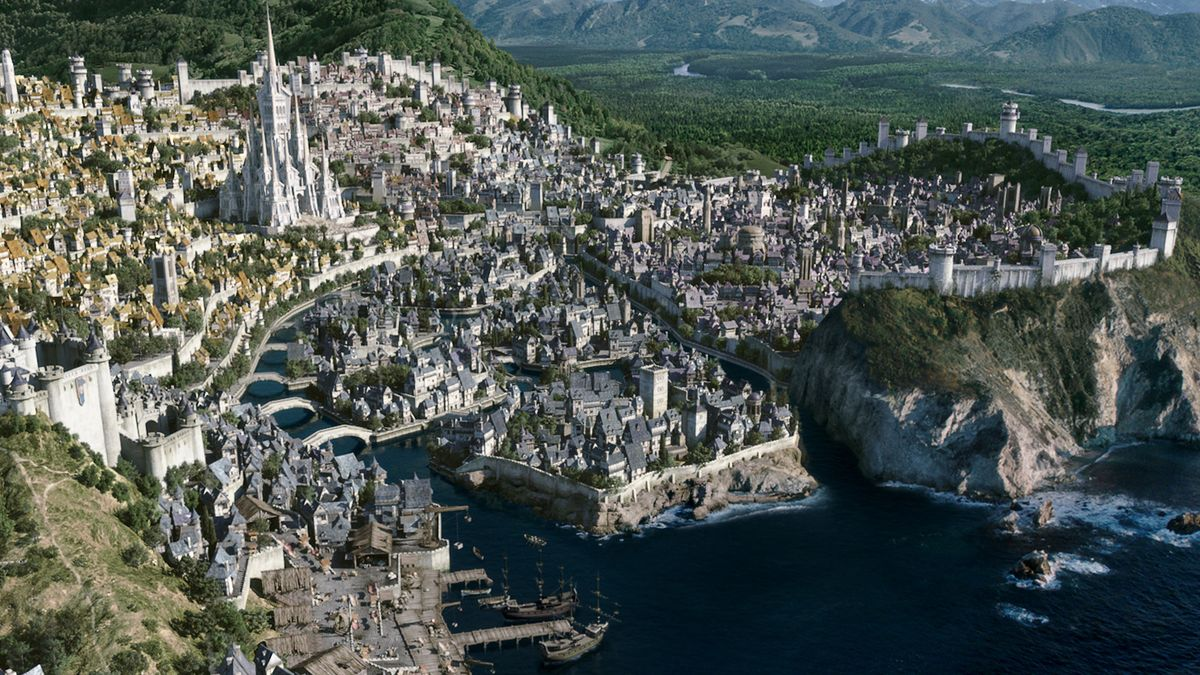
\includegraphics[width=\linewidth]{img/WoW/1200px-StormwindPanorama.jpg}
	
	{Tempestas: Tempestas is a marvelous sight.}
\end{center}

\section{Tempestas}
\begin{center}
	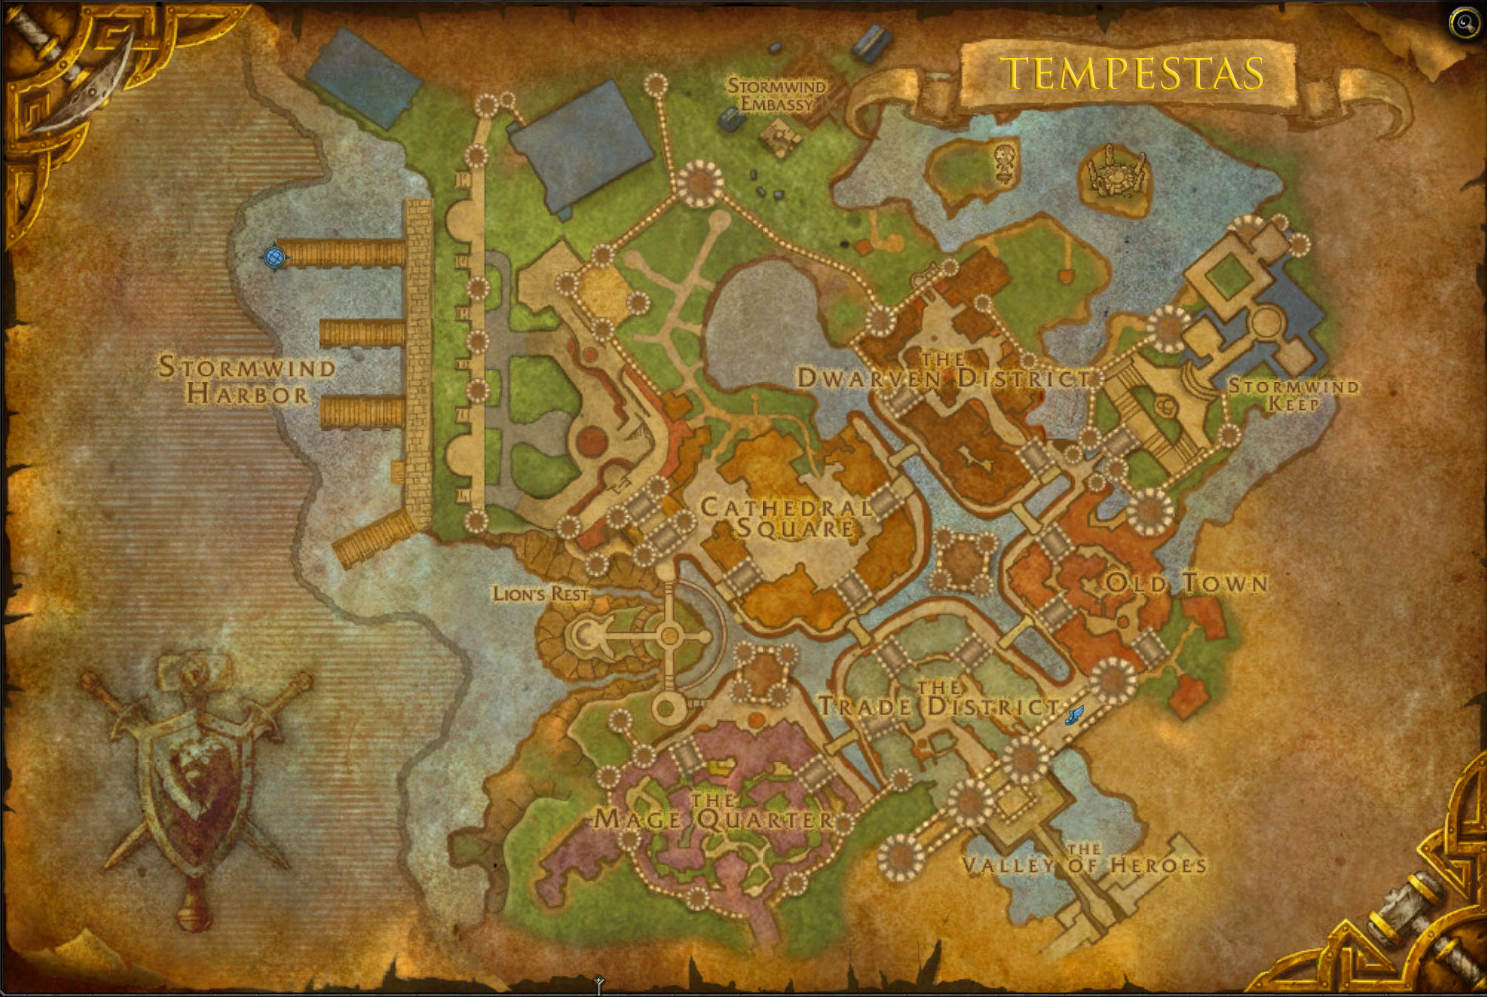
\includegraphics[width=\linewidth]{img/maps/Tempestas.jpg}
	
	{\textbf{Tempestas:} The main trading post of the south west region of the planet. Everything can be found here from crime, to various trade skills.}
\end{center}

\begin{center}
	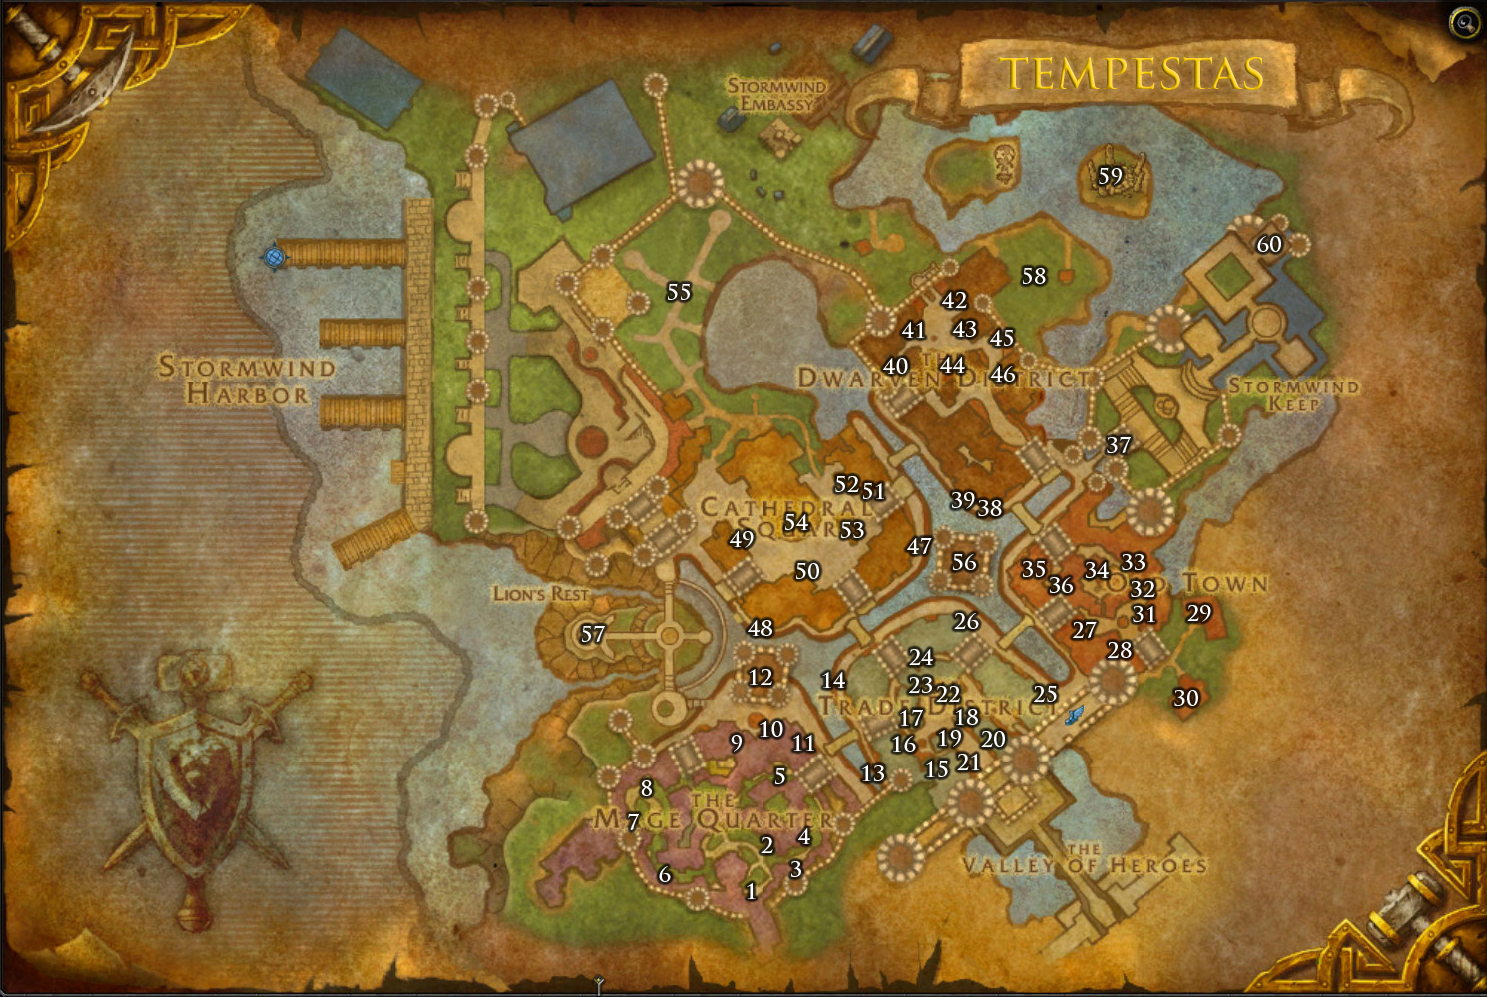
\includegraphics[width=\linewidth]{img/maps/Tempestas_labeled.jpg}
	
	{\begin{multicols}{3}
		\begin{enumerate}
			\item The Blue Recluse (Tavern)
			\item Larson Clothiers
			\item Alchemy Needs
			\item Duncan's Textiles
			\item Tempestas Staves
			\item Ancient Curios
			\item The Slaughtered Lamb (Pub)
			\item Pyrotechnics
			\item The Scribe of Tempestas
			\item Academy of Arcane Arts
			\item Cordell's Enchanting
			\item Tempestas Prison
			\item Gallina Winery
			\item Canal Tailor and Fit shop
			\item Tempestas Counting House (Bank)
			\item The Gilded Rose (Inn)
			\item Tempestas Trade House
			\item Everyday Merchandise
			\item Pestle's Apothecary
			\item Trias' Cheese
			\item Tempestas Visitor's Center
			\item Weller's Arsenal
			\item Lionheart Armory
			\item Barbara's Barbor
			\item Fragrant Flowers
			\item Denman Family Jewelers
			\item The Protective Hide
			\item Champion's Hall
			\item SI:7
			\item Command Center
			\item Limited Immunity (Armors)
			\item Honest Blades
			\item Pig \& Whistle Tavern
			\item Heavy Handed Weapons
			\item The Silver Shield
			\item Thane's Boots
			\item Tempestas Keep
			\item Pott's Plates
			\item The Shady Lady
			\item Stonehand Mining
			\item Auction House
			\item Royal Bank of Tempestas
			\item The Golden Keg (Tavern)
			\item Engineering Ward
			\item Deeprun Tram
			\item Hunters Hovel
			\item Ol' Emmas
			\item The Three Winds
			\item Just Maces
			\item Rightous Plates
			\item The Argent Dawn
			\item City Hall
			\item Orphanage
			\item Cathedral
			\item Graveyard
			\item Maximum Security
			\item Varian Wrynn Memorial
			\item Audrey Burnhep
			\item Earthshrine
			\item Royal Library
		\end{enumerate}
	\end{multicols}}
\end{center}

\subsection{Tempestas Hierarchy}

Within Tempestas, there is a hierarchy of power and rule. The Hierarchy of who is in charge is as follows.
\begin{enumerate}
	\item King and Queen.
	\begin{enumerate}
		\item The King is at the head of the City. He controls the military and decisions of the Nobles. His family is at the head of the government and economic system in Tempestas.
	\end{enumerate}
	\item Royal Advisory.
	\begin{enumerate}
		\item Royal Guard. The Royal Guard is the Kings personal protection for him and his family. These guards are specially trained in matters of combat and intelligence.
		\item Royal Council. The Royal Council is a group of wise men and advisors that the King uses in making decisions pertaining to the times. These include Daniel the Prophet, Kinsey the military advisor, Turelyon the religious advisor, and Nicholas the economic advisor. 
	\end{enumerate}
	\item Nobles
	\begin{enumerate}
		\item Nobles. The Nobles are the rich elite that control different sub-sections of the city. There are seven Nobles in total which each essentially control a different part of the city.
		\begin{enumerate}
			\item Sir Francis Lancelot. He is head over the Trade district. He is the big economic power in Tempestas as he controls teh trade markets and the banking system. He oversees a Nobles vault within the bank which is like a security deposit system for rare and valuable items.
			\item Saint Palagius the Wise. This is the Noble overhead of the Cathedral Square and all of its businesses. This includes the Cathedral and Graveyard of Tempestas.
			\item Delgore Zuba de Hut. This is the Noble overhead of the Storm wind Harbor. He has control over trade and harbor security. When the city is in lock down, the only way to enter or leave is through his permission or the Kings. 
			\item Gimley Bronzebeard. This is the Noble over the Dwarven District. He is head of the Brawler's Guild which is an underground club where the black market is located and run.
			\item Others
		\end{enumerate}
		\item Noble Families. Right below the Nobles, the Noble families have a large amount of power just through affiliation with the Nobles.
		\item Noble Guards. Since the Nobles have a vast amount of power and money, they have their own guards and watch over different parts of the cities. The King is ahead of all of these troops in times of National security but in general they are lead by the Noble above them.
		\item Noble Councils. The Nobles generally have their own councils and workers directly under them.
	\end{enumerate}
	\item Tempestas Officials.
	\begin{enumerate}
		\item Mayor. This is the head of civil affairs. He has minor control over laws and resources used throughout the city.
		\item District leaders. These are generally appointed by the Nobles (indirectly) through a 'democratic' voting system. They are in charge of affairs relating to the businesses throughout each sector.
		\item Trade leaders. These are the head business men in each division (trade, religion, crafting, etc).
		\item Tempestas Guards. These are normal guards appointed to be on duty throughout the city. Much like a police force.
	\end{enumerate}
	\item Shop keepers.
	\item Citizens.
\end{enumerate}

\subsection{Brawlers Guild}

The Brawlers guild is a secret underground club that was created by black market leaders and allowed to exist by the Nobles. Any corrupt business dealings will generally go on here as it is privately guarded with Mercenary bouncers. Entrance to the Brawlers Guild requires a scroll of approval (Brawlers pass) with the signatures of the Brawler officials. These passes are hard to obtain and generally extremely expensive. Within the Brawlers guild is an underground sand arena where fights and battles are waged. There is a custom orchestra playing music for the fights and bets are placed on the battles. The champion of the arena (Jay Maul) is essentially Darth Maul from Star Wars only wields a duel bladed stave with electrical capabilities. He is an agile fighter who makes many small attacks quickly in succession and is hard to hit.







